\chapter{Clipping}

Wenn man in einem Raum auf ein Objekt schaut, so sieht man nur z.B. nur einen Teil davon. Der andere Teil wäre schon da, ist aber nicht sichtbar. In einer 3D Rendering Engine wäre es jetzt unnötig, dazu alle Lichteffekt usw. schon zu berechnen, deswegen schneidet man es weg. Das nennt man Clipping.

\section{3D vs 2D Clipping}
Clipping geschieht in mehreren Stufen. Nachdem die 3D Szene aufgebaut ist, werden 3D Objekte entfernt, welche z.B. nicht im View Bereich der Kamera sind. Das wäre 3D Clipping. 2D Clipping bedeutet, dass nachdem alle Beleuchtung usw. berechnet wurde, noch der Teil rausgeschniten wird, der nicht auf den Bildschirm passt - bevor das Bild dann schlussendlich gerastert und dargestellt wird.
\begin{figure}[!ht]
	\centering
	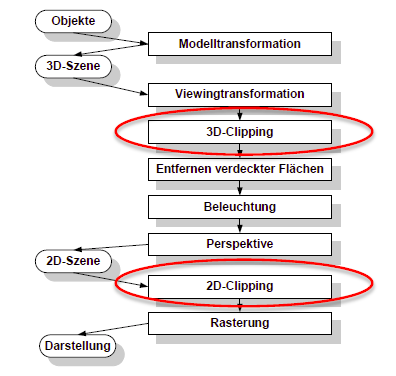
\includegraphics[width=0.4\linewidth]{fig/grafikpipeline}
	\caption{Grafikpipeline}
	\label{fig:grafikpipeline}
\end{figure}

\section{Clipping Variationen}
Man kann auf verschiedene Arten allgemein nun Clippen (3D).
\begin{enumerate}
	\item \textbf{Scissering} \\
	Die 'dümmste' Variante des Clippings. Hier wird das 3D Clipping einfach übersprungen und nur am Schluss einfach die gezeichnet, welche gerade so im Fenster liegen.
	\item \textbf{Temporärer Buffer} \\
	Das gesamte Objekt wird auf Vorrat in einem temporären Buffer gezeichnet, welcher bei der Verwendung des Zeichenobjekts ins Zielbild kopiert wird. 
	Dieses Verfahren wird beispielsweise für Buchstaben einer Schrift angewandt. Da die Objekte nicht mehr Polygone sondern fertig gezeichnetes Bilder sind, lassen sich dieses sehr einfach schneiden.
	\item \textbf{Analytische Berechnung} \\ 
	Man berechnet irgendwie, was darin liegt. Man siehe unten.
\end{enumerate}

\section{Linien Clipping}
Gehen wir von einem ganz einfachen Fall aus - dem Clipping einer Linie. Wir haben also ein Rechteck, welches z.B. den Canvas darstellt. Hindurch geht eine Linie. Wir möchten nun berechnen, welche Punkte gezeichnet werden müssen, resp. eine Linie haben, welche genau innerhalb des gezeichneten Rechtecks ist. Dazu gibt es die nachfolgenden Varianten.

\subsection{Brute Force}
Wenn mindestens ein Endpunkt der Linie ausserhalb des Rechtecks liegt (also wenn die Linie einfach etwas herausgeht aus dem Rechteck), dann müsste man alle Schnittpunkte berechnen, die die Linie mit dem Kappungs-Rechteck hat. Das scheint aber für CG Anwendungen zu unperformant zu sein.

\subsection{Cohen-Sutherland}
Nette Herren, die sich folgende Methode ausgedacht haben:
\begin{enumerate}
	\item Nimm den Anfangs- \& Endpunkt der Linie. Schau, in welchem Bereich der Punkt liegt:
	
	\begin{figure}[!ht]
		\centering
		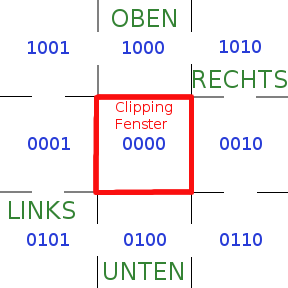
\includegraphics[width=0.3\linewidth]{fig/cohen_sutherland}
		\caption{Bereiche der Grafik für den Algorithmus von Cohen Sutherland}
		\label{fig:cohen_sutherland}
	\end{figure}
	
	Liegt der Punkt oben rechts vom Clipping Fenster, so hat der Punkt den Wert \textit{1010}. Ist er rechts unten, so ist der Wert \textit{0110}. Der Wert wird also bitweise bestimmt, in der Reihenfolge:
	\begin{enumerate}
		\item Oben (1000)
		\item Unten (0100)
		\item Rechts (0010)
		\item Links (0001)
	\end{enumerate}
	\item Ist der Code bei beiden Punkten \textit{0000}, so liegen ja beide Punkte im Clipping Fenster und die Linie wird akzeptiert und so gezeichnet.
	\item Ansonsten wird Bit für Bit der Wert verglichen und geschaut, ob bei beiden der Wert 1 ist. Das heisst es wird das erste Bit genommen, dann das zweite usw. Eigentlich wird geschaut, ob beide Punkte links, rechts, oben oder unten des Rechtsecks sind. Denn wenn das der Fall ist, so geht die Linie nämlich sicher nicht durch das Clipping Fenster und die Linie kann abgelehnt werden.
	\item Wenn die Linie aber durch das Vergleichen nicht abgelehnt werden konnte, so wird der Schnittpunkt mit einer beliebigen Seite des Clipping Fensters berechnet und die Linie so \textit{entzweigeschnitten}. Einen Teil der Linie kann dann verworfen werden, der andere Teil der Linie wird nochmals durch den Algorithmus gejagt, bis dann alles im Rechteck vorhanden ist.
\end{enumerate}

\section{Polygone Clippen}
Das wird schon etwas aufwändiger. Wir haben hier einen Algorithmus von den Herren \textbf{Sutherland-Hodgeman}, der eigentlich nur für Geraden geht - aber da ein Rechteck ja eigentlich einfach aus 4 Geraden besteht, machen wir das Ganze einfach 4x - dann passts auch.

Ein Polygon besteht ja aus n-Punkten. Wir gehen jetzt von einem Startpunkt aus und gehen dann von Punkt zu Punkt. Wir schauen dann jeweils einfach für den Startpunkt \textit{S} und den nächsten Punkt des Polygons \textit{P}, ob diese Punkte innerhalb oder ausserhalb des Polygons liegen. Dies wird für alle Punkte gemacht, das heisst jeder Punkt ist mal Startpunkt und jeder Punkt ist mal Endpunkt. Die Ausgabe des Algorithmus bestimmt dann, welcher Punkt behalten wird. Wenn die Punkte die Linien schneiden, wird einfach der Schnittpunkt dazu berechnet und entsprechend auch gespeichert.
	
\begin{figure}[!ht]
	\centering
	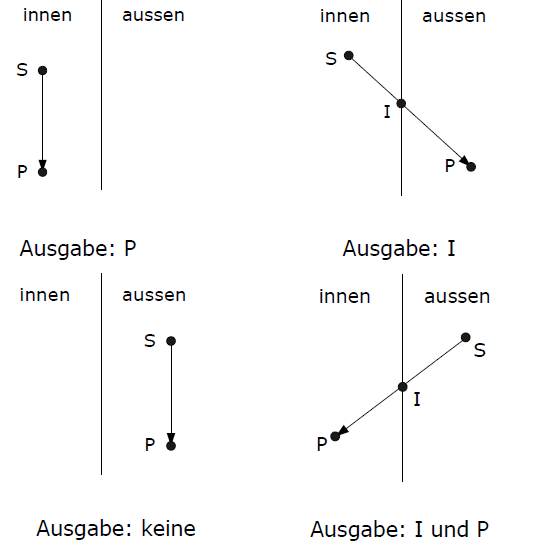
\includegraphics[width=0.5\linewidth]{fig/sutherland_hodgman}
	\caption{Verschiedene Fälle für den Sutherland Hodgman Algorithmus}
	\label{fig:sutherland_hodgman}
\end{figure}